\subsection{Intel Top-Down Classification}
\label{sec:topdown}

Intel Top-Down (ITD)~\cite{Yasin:2014:TDM} classifies pipeline activity very broadly into four categories: \textbf{frontend bound}, \textbf{bad speculation}, \textbf{retiring}, and \textbf{backend bound} (see Figure~\ref{fig:topdown2}). Each of these categories can be broken down even further and differently depending on the architecture. Below we describe the four top-level categories for the LEON3 (32-bit SPARC V8 architecture) instruction pipeline since this is the architecture used in our measurements.

\textbf{Frontend Bound.} The frontend includes the front portion of the pipeline where the branch predictor predicts the next address, instructions are fetched and decoded, and the register file is accessed. The frontend prepares instructions to be executed by the backend of the processor. Cycles are classified as frontend bound when the frontend undersupplies the backend of the pipeline (e.g. instruction cache misses).

\textbf{Bad speculation.} This category captures inefficiency in the pipeline due to incorrect speculation by the branch predictor. This includes issued instructions that do not eventually get retired. These instructions are annulled (i.e. has no effect and effectively not executed) in the LEON3.  

\textbf{Retiring.} This category is for issued instructions that eventually get retired. 

\textbf{Backend Bound.} A cycle is classified as backend bound when a new instruction is not issued to the execution unit in a given cycle while the frontend of the pipeline is not stalled. This may be due to data cache misses or overloaded functional units. The backend category can be further broken down into \emph{core bound} and \emph{memory bound}. 

\begin{itemize}
\item [--] \underline{Core bound} includes stalls due to overloaded functional units.
\item [--] \underline{Memory bound} includes store bound (i.e. high number of buffered stores), L1 bound (cache access), and memory bound (cache miss).
\end{itemize}

\begin{figure}[htbp]
  \begin{center}
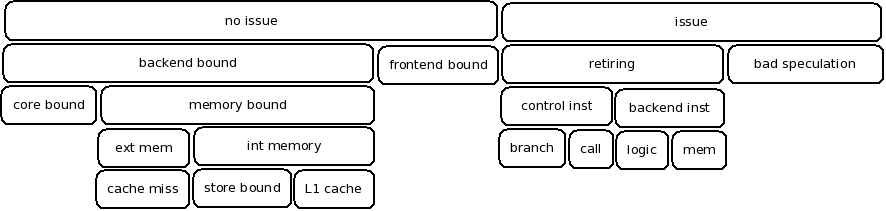
\includegraphics[width=0.99\columnwidth]{figs/topdown2}
  \end{center}
  \caption{An example of the Intel Top-Down processor activity categories.}
  \label{fig:topdown2}
\end{figure}

Traditionally, the ITD categories has been used for the purpose of detecting sources of performance bottlenecks. The motivation for using the ITD classification to detect SFG phases is that the different categories provides different levels of detail regarding pipeline activity, which we think is a good model for program behavior. Furthermore, hardware complexity is significantly reduced since only a finite vector of size $n$ is necessary to store the frequency of each category over an interval, where $n$ is the number of categories at each level. By comparison, the hardware complexity is a function of the number of unique instructions in the case of IWS and the number of unique basic blocks in the case of BBVs, which can be difficult to determine a priori. The ITD vector difference between intervals is computed using the Manhattan distance, similar to the BBV difference.



